\section{Métricas} % Seções são adicionadas para organizar sua apresentação em blocos discretos, todas as seções e subseções são automaticamente exibidas no índice como uma visão geral da apresentação, mas NÃO são exibidas como slides separados.

%----------------------------------------------------------------------------------------

\begin{frame}
    \only<1-4>{
        \frametitle{ROUGE}
        \begin{itemize}[<+(1)->]
            \item Proposto por Lin et al. em 2004
            \item Faz uso de n-gramas
            \item É uma métrica baseada no Recall.
        \end{itemize}
    }
    \only<5>{
        \frametitle{ROUGE-N}
        \begin{equation} \tag{1}
            \label{eq:rouge-n-1}
            \text{Match}(\text{g}) =
            \min\left(\text{count}_{\text{ref}}(\text{g}), \text{count}_{\text{pred}}(\text{g}) \right)
        \end{equation}

        \begin{equation}
            \label{eq:rouge-n-2} \tag{2}
            \text{ROUGE-N} = 
            \frac{
            \sum_{\text{n-gram} \in ref}
            \text{Match}(\text{n-gram})
            }{
            \sum_{\text{n-gram} \in ref} \text{count}_{\text{ref}}(\text{n-gram})
            }
        \end{equation}
    }
    \only<6>{
        \frametitle{ROUGE-L}
        \begin{equation} \tag{1}
            \label{eq:rouge-l1} 
            R_{\text{LCS}} = \frac{ \text{LCS}(ref, pred) }{ ||ref|| }
            \quad\text{e}\quad
            P_{\text{LCS}} = \frac{ \text{LCS}(ref, pred) }{ ||pred|| }
        \end{equation}

        \begin{equation}
            \label{eq:rouge-l2} \tag{2}
            \text{ROUGE-L} =
            \frac{ 2 \cdot R_{\text{LCS}} \cdot P_{\text{LCS}} }
            { R_{\text{LCS}} + \cdot P_{\text{LCS}} }
        \end{equation}
    }
\end{frame}

%----------------------------------------------------------------------------------------

\begin{frame}
    \frametitle{BLEU}
    \only<1-6>{
        \begin{itemize}[<+(1)->]
            \item Proposto por Papineni et al. em 2002
            \item Focada em Tradução
            \item Faz uso de n-gramas
            \item É uma métrica baseada no Precisão
            \item Possui punição por brevidade
        \end{itemize}
    }
    \only<7>{
        \begin{equation} \tag{1}
            \label{eq:precisionBLEU-1}
            \text{Match}(\text{g}) =
            \min\left(\text{count}_{\text{pred}}(\text{g}), \text{count}_{\text{ref}}(\text{g}) \right)
        \end{equation}

        \begin{equation} \tag{2}
            \label{eq:precisionBLEU-2}
            P_n = \frac{
            \sum_{\text{n-gram} \in pred} \text{Match}(\text{n-gram})
            }{
            \sum_{\text{n-gram} \in pred} \text{count}_{pred}(\text{n-gram})
            }
        \end{equation}
    }
    \only<8>{
        \begin{equation} \tag{1}
            \label{eq:penalidadeBLEU}
            \text{BP} = 
            \begin{cases}
                1, & \text{se } ||pred|| > ||ref|| \\
                e^{1 - \frac{||ref||}{||pred||}}, & \text{se } ||pred|| \leq ||ref||
            \end{cases}
        \end{equation}

        \begin{equation} \tag{2}
            \label{eq:BLEUval}
            \text{BLEU} = \text{BP} \times \exp\left( \sum_{n=1}^N w_n \log P_n \right)
        \end{equation}

        \vspace{30px}

        $w_n$ = $\frac{1}{n}$
    }
    
\end{frame}

%----------------------------------------------------------------------------------------
\begin{frame}
    \frametitle{METEOR}
    \only<1-6>{
        \begin{itemize}[<+(1)->]
            \item Proposto por Banerjee et al. em 2005
            \item Focada em Tradução
            \item Faz uso de unigramas
            \item Aceita sinônimos e variações morfológicas simples
            \item Possui punição com base no ordenamento das palavras
        \end{itemize}
    }
    \only<7>{
        \begin{equation} \tag{1}
            \label{eq:METEORp}
            P = \frac{\text{\#1-grams}}{||pred||}, \quad R = \frac{\text{\#1-grams}}{||ref||} \quad e \quad F_{\alpha} = \frac{P \cdot R}{\alpha \cdot P + (1 - \alpha) \cdot R}
        \end{equation}

        \begin{equation} \tag{2}
            \label{eq:METEORpenalidade}
            \text{Penalidade} = \gamma \cdot \left(\frac{\text{\#chunks}}{\text{\#1-grams}}\right)^{\beta}
        \end{equation}

        \begin{equation} \tag{3}
            \label{eq:METEORval}
            \text{METEOR} = (1 - \text{Penalidade}) \cdot F_{\alpha}
        \end{equation}

        \vspace{30px}

        $\alpha$ = 0.90 \\
        $\beta$  = 3.00 \\ 
        $\gamma$ = 0.50
    }
\end{frame}

%----------------------------------------------------------------------------------------

\begin{frame}
    \frametitle{BERTScore}
    \only<1-5>{
        \begin{itemize}[<+(1)->]
            \item Proposto por Zhang et al. em 2019
            \item Faz uso de PLMs (Modelo BERT)
            \item Cria embeddings contextuais das palavras
            \item Calcula a distância de cosseno entre elas
        \end{itemize}
    }
    \only<6>{
        \begin{figure}
            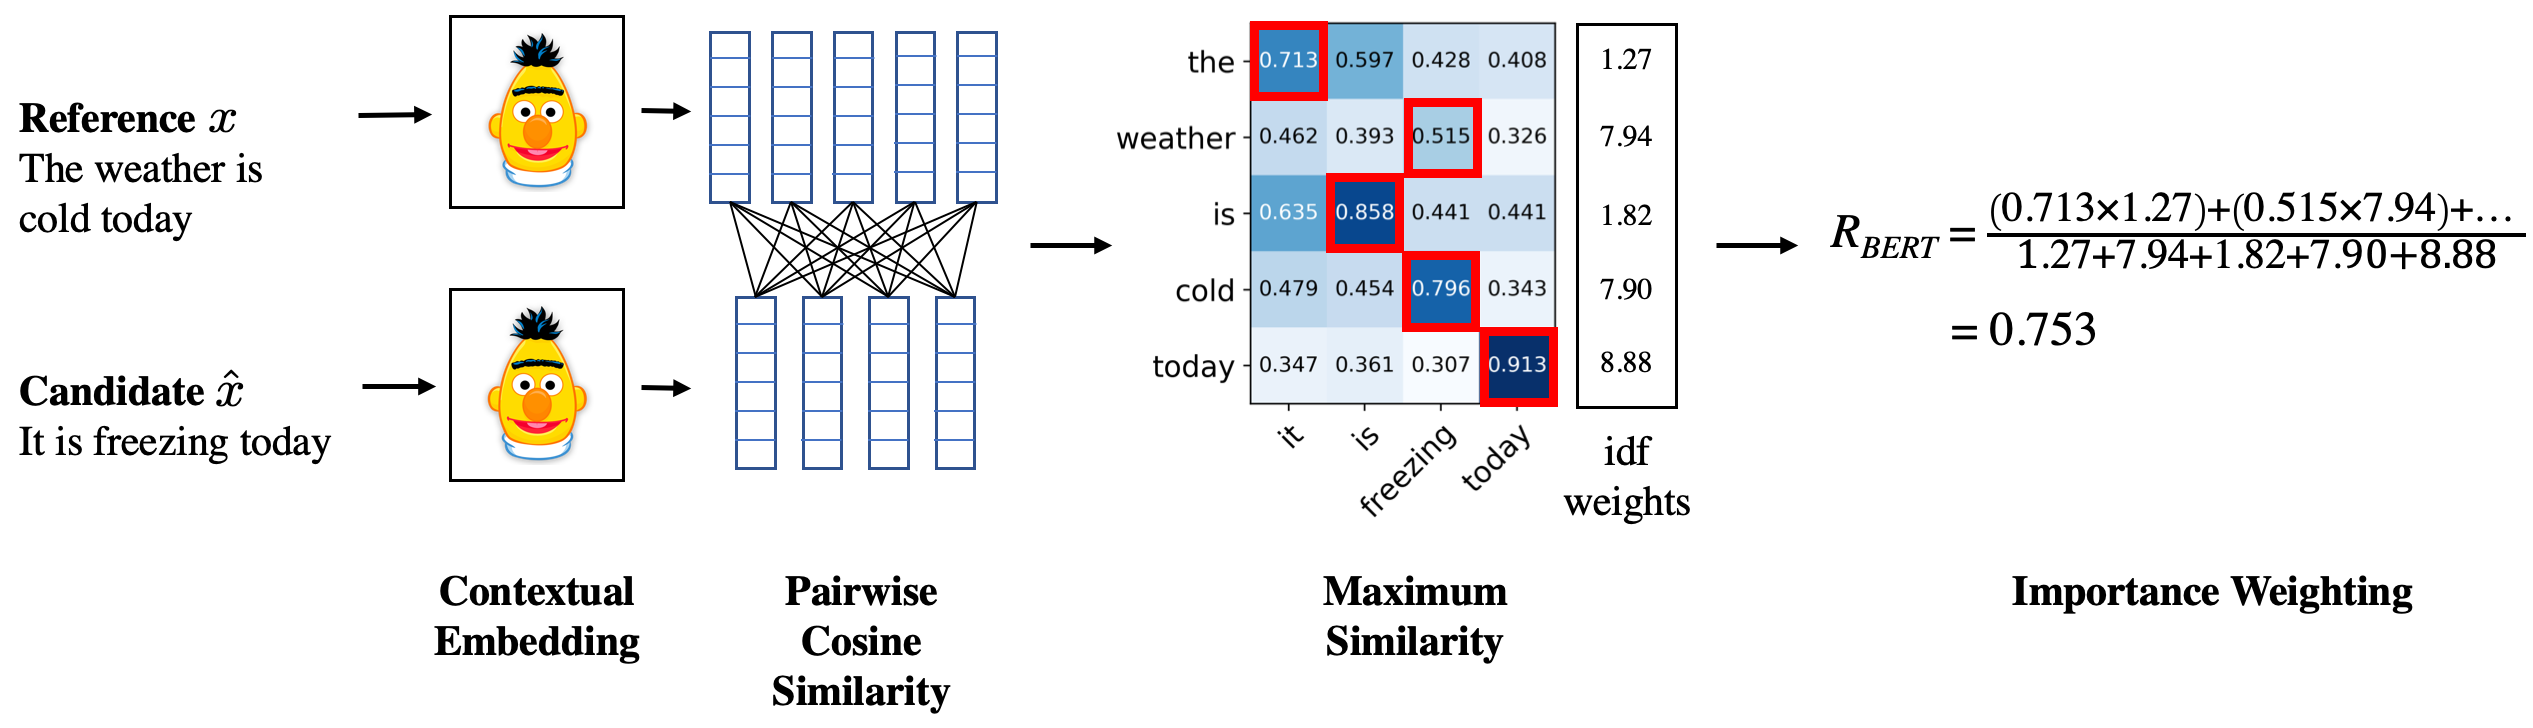
\includegraphics[width=\textwidth]{bert_score.png}
            % \caption{Fonte: \citet{bert-score}.}
        \end{figure}
    }
    \only<7>{
        \begin{equation} \tag{1}
            \label{eq:BERTScore-pr-1}
            P = \frac{1}{||pred||} \sum_{i=1}^{||pred||} \max_{j \in [1, ||ref||]} \text{Sim}(\text{pred}_i, \text{ref}_j)
        \end{equation}

        \begin{equation} \tag{2}
            \label{eq:BERTScore-pr2}
            R = \frac{1}{||ref||} \sum_{j=1}^{||ref||} \max_{i \in [1, ||pred||]} \text{Sim}(\text{ref}_j, \text{pred}_i)
        \end{equation}

        \begin{equation} \tag{3}
            \label{eq:BERTScore-f1}
            F_1 = \frac{2 \cdot P \cdot R}{P + R}
        \end{equation}
    }
\end{frame}

%----------------------------------------------------------------------------------------

\begin{frame}
    \frametitle{BARTScore}
    \only<1-4>{
        \begin{itemize}[<+(1)->]
            \item Proposto por Yuan et al. em 2021
            \item Faz uso de PLMs (Modelo BART)
            \item Calcula a probabilidade logaritmica de que o modelo BART gere a saída 
            dado um texto base
        \end{itemize}
    }
    \only<5->{
        \begin{equation} \tag{1}
            \label{eq:BARTScore-p}
            P = \text{Prob}_\text{Geração}(ref \rightarrow pred)
        \end{equation}

        \begin{equation} \tag{2}
            \label{eq:BARTScore-r}
            R = \text{Prob}_\text{Geração}(pred \rightarrow ref)
        \end{equation}

        \begin{equation} \tag{3}
            \label{eq:BARTScore-f1}
            F_1 = \frac{P + R}{2}
        \end{equation}
    }
\end{frame}

%----------------------------------------------------------------------------------------

\begin{frame}
    \frametitle{MoverScore}
    \only<1-7>{
        \begin{itemize}[<+(1)->]
            \item Proposto por Zhao et al. em 2019
            \item Faz uso de PLMs (Normalmente BERT)
            \item Realiza embedding contextial das palavras do texto
            \item Atribui às palavras um peso de importância baseado no TF-IDF
            \item Calcula o custo mínimo para alinhar os vetores
            \item Faz uso do Word Mover's Distance
        \end{itemize}
    }
    \only<8>{
        \begin{figure}
            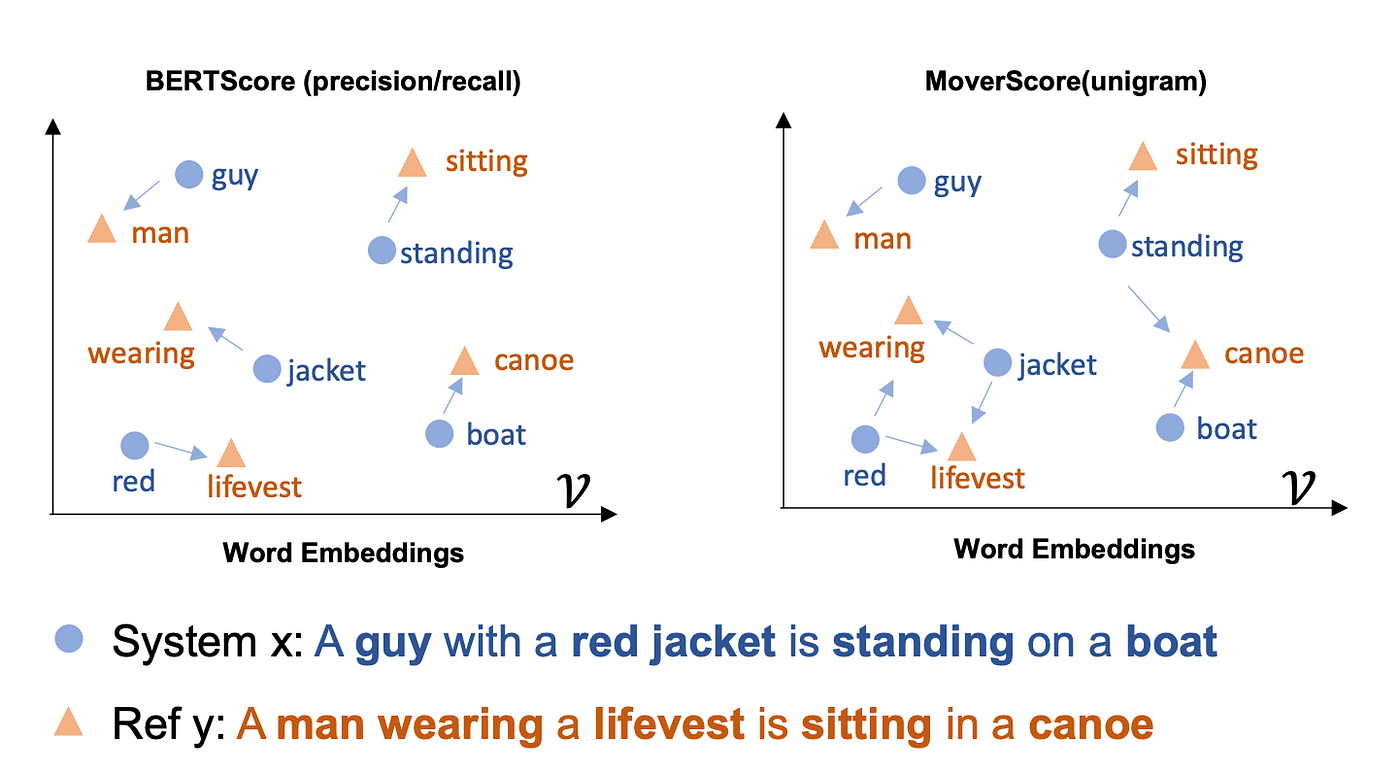
\includegraphics[width=0.8\textwidth]{moverscore.png}
            % \caption{Fonte: \citet{bert-score}.}
        \end{figure}
    }
\end{frame}